%==============================================================================
% Figure: Quantum Foam Interferometer
% Purpose: Michelson interferometer for quantum foam detection
% Chapter: Ch24 - Quantum Foam Experimental Protocols
% Type: Schematic
%==============================================================================

\begin{figure}[htbp]
  \centering
  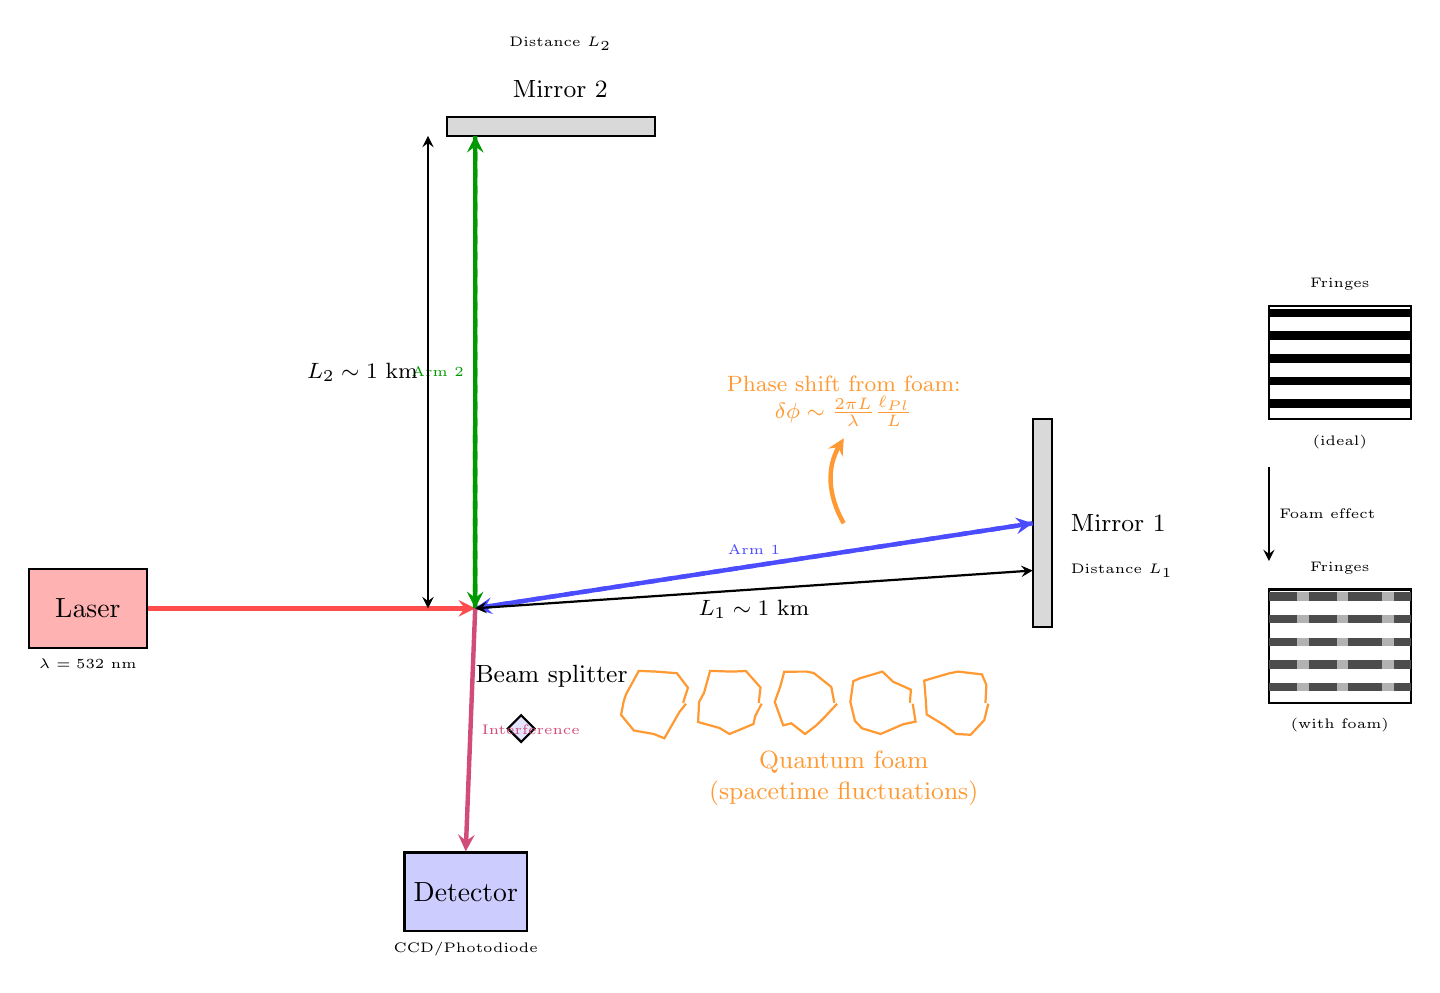
\begin{tikzpicture}[
    scale=1.2,
    mirror/.style={thick, draw=black, fill=gray!30},
    beam/.style={ultra thick, ->, >=stealth},
    detector/.style={rectangle, draw=black, fill=blue!20, thick, minimum width=1cm, minimum height=1cm}
  ]

    %========== Laser Source ==========
    \node[rectangle, draw=black, fill=red!30, thick, minimum width=1.5cm, minimum height=1cm]
      (laser) at (-6, 0) {Laser};
    \node[font=\tiny, below] at (laser.south) {$\lambda = 532$ nm};

    %========== Beam Splitter ==========
    \draw[mirror, fill=blue!10, rotate=45] (-2, 0) rectangle (-1.8, 0.2);
    \node[font=\small, below right] at (-2, -0.5) {Beam splitter};
    \coordinate (BS) at (-1.9, 0);

    %========== Mirrors ==========
    % Horizontal arm mirror
    \draw[mirror] (4, -0.2) rectangle (4.2, 2);
    \node[font=\small, right] at (4.3, 0.9) {Mirror 1};
    \node[font=\tiny, right] at (4.3, 0.4) {Distance $L_1$};

    % Vertical arm mirror
    \draw[mirror] (-2.2, 5) rectangle (0, 5.2);
    \node[font=\small, above] at (-1, 5.3) {Mirror 2};
    \node[font=\tiny, above] at (-1, 5.8) {Distance $L_2$};

    %========== Detector ==========
    \node[detector] (det) at (-2, -3) {Detector};
    \node[font=\tiny, below] at (det.south) {CCD/Photodiode};

    %========== Laser Beam Paths ==========
    % Incident beam to beam splitter
    \draw[beam, red!70] (laser.east) -- (BS);

    % Transmitted beam to Mirror 1 (horizontal arm)
    \draw[beam, blue!70] (BS) -- (4, 0.9) node[midway, above, font=\tiny] {Arm 1};

    % Reflected beam to Mirror 2 (vertical arm)
    \draw[beam, green!60!black] (BS) -- (-1.9, 5) node[midway, left, font=\tiny] {Arm 2};

    % Return beam from Mirror 1
    \draw[beam, blue!70, dashed] (4, 0.9) -- (BS);

    % Return beam from Mirror 2
    \draw[beam, green!60!black, dashed] (-1.9, 5) -- (BS);

    % Recombined beam to detector
    \draw[beam, purple!70] (BS) -- (det.north) node[midway, right, font=\tiny] {Interference};

    %========== Quantum Foam (wavy spacetime) ==========
    % Schematic foam around horizontal arm
    \foreach \x in {0, 0.8, 1.6, 2.4, 3.2} {
      \draw[orange!80, thick, decorate, decoration={random steps, segment length=2mm, amplitude=1mm}]
        (\x, -1) circle (0.3cm);
    }
    \node[font=\small, text=orange!80, align=center] at (2, -1.8) {Quantum foam\\(spacetime fluctuations)};

    %========== Phase Shift Annotation ==========
    \draw[->, >=stealth, ultra thick, orange!80] (2, 0.9) to[bend left=30] (2, 1.8)
      node[above, align=center, font=\footnotesize] {
      Phase shift from foam: \\
      $\delta\phi \sim \frac{2\pi L}{\lambda} \frac{\ell_{\text{Pl}}}{L}$
    };

    %========== Arm Length Labels ==========
    \draw[<->, >=stealth, thick] (BS) -- (4, 0.4) node[midway, below, font=\footnotesize] {$L_1 \sim 1$ km};
    \draw[<->, >=stealth, thick] (-2.4, 0) -- (-2.4, 5) node[midway, left, font=\footnotesize] {$L_2 \sim 1$ km};

    %========== Interference Pattern (inset) ==========
    \begin{scope}[shift={(6.5, 2)}, scale=0.6]
      \draw[thick] (0, 0) rectangle (2.5, 2);
      \foreach \y in {0.2, 0.6, 1.0, 1.4, 1.8} {
        \fill[black] (0, \y) rectangle (2.5, {\y + 0.15});
      }
      \node[font=\tiny, above] at (1.25, 2.1) {Fringes};
      \node[font=\tiny, below] at (1.25, -0.1) {(ideal)};
    \end{scope}

    \begin{scope}[shift={(6.5, -1)}, scale=0.6]
      \draw[thick] (0, 0) rectangle (2.5, 2);
      \foreach \y in {0.2, 0.6, 1.0, 1.4, 1.8} {
        \fill[black!70] (0, \y) rectangle (2.5, {\y + 0.15});
        % Add random perturbations
        \fill[black!30] (0.5, \y) rectangle (0.7, {\y + 0.15});
        \fill[black!30] (1.2, \y) rectangle (1.4, {\y + 0.15});
        \fill[black!30] (2.0, \y) rectangle (2.2, {\y + 0.15});
      }
      \node[font=\tiny, above] at (1.25, 2.1) {Fringes};
      \node[font=\tiny, below] at (1.25, -0.1) {(with foam)};
    \end{scope}

    \draw[->, >=stealth, thick] (6.5, 1.5) -- (6.5, 0.5) node[midway, right, font=\tiny] {Foam effect};

  \end{tikzpicture}

  \vspace{0.5cm}

  %========== Explanation Boxes ==========
  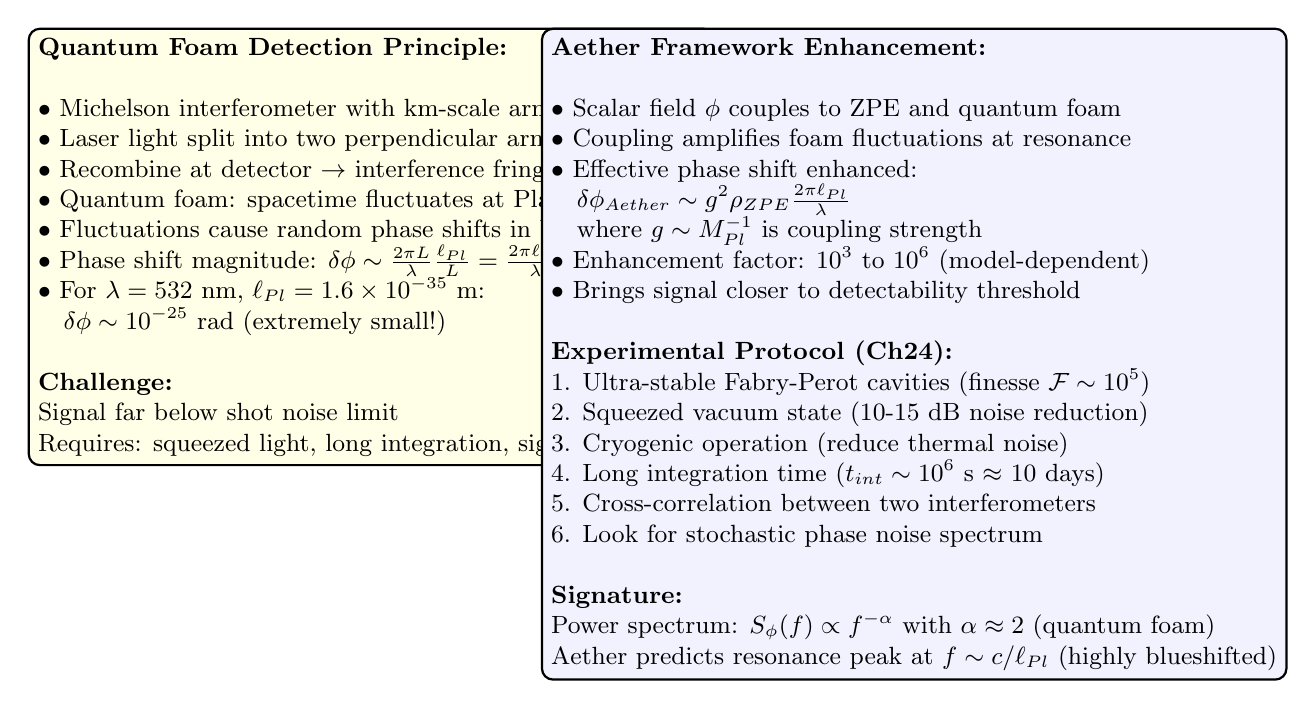
\begin{tikzpicture}
    \node[anchor=north west, align=left, font=\small, draw=black, fill=yellow!10, rounded corners, thick]
      at (0, 0) {
      \textbf{Quantum Foam Detection Principle:} \\
      \\
      $\bullet$ Michelson interferometer with km-scale arms ($L \sim 1$ km) \\
      $\bullet$ Laser light split into two perpendicular arms \\
      $\bullet$ Recombine at detector $\to$ interference fringes \\
      $\bullet$ Quantum foam: spacetime fluctuates at Planck scale $\ell_{\text{Pl}}$ \\
      $\bullet$ Fluctuations cause random phase shifts in beam paths \\
      $\bullet$ Phase shift magnitude: $\delta\phi \sim \frac{2\pi L}{\lambda} \frac{\ell_{\text{Pl}}}{L} = \frac{2\pi\ell_{\text{Pl}}}{\lambda}$ \\
      $\bullet$ For $\lambda = 532$ nm, $\ell_{\text{Pl}} = 1.6 \times 10^{-35}$ m: \\
      \quad $\delta\phi \sim 10^{-25}$ rad (extremely small!) \\
      \\
      \textbf{Challenge:} \\
      Signal far below shot noise limit \\
      Requires: squeezed light, long integration, signal processing
    };

    \node[anchor=north east, align=left, font=\small, draw=black, fill=blue!5, rounded corners, thick]
      at (16, 0) {
      \textbf{Aether Framework Enhancement:} \\
      \\
      $\bullet$ Scalar field $\phi$ couples to ZPE and quantum foam \\
      $\bullet$ Coupling amplifies foam fluctuations at resonance \\
      $\bullet$ Effective phase shift enhanced: \\
      \quad $\delta\phi_{\text{Aether}} \sim g^2 \rho_{\text{ZPE}} \frac{2\pi\ell_{\text{Pl}}}{\lambda}$ \\
      \quad where $g \sim M_{\text{Pl}}^{-1}$ is coupling strength \\
      $\bullet$ Enhancement factor: $10^3$ to $10^6$ (model-dependent) \\
      $\bullet$ Brings signal closer to detectability threshold \\
      \\
      \textbf{Experimental Protocol (Ch24):} \\
      1. Ultra-stable Fabry-Perot cavities (finesse $\mathcal{F} \sim 10^5$) \\
      2. Squeezed vacuum state (10-15 dB noise reduction) \\
      3. Cryogenic operation (reduce thermal noise) \\
      4. Long integration time ($t_{\text{int}} \sim 10^6$ s $\approx$ 10 days) \\
      5. Cross-correlation between two interferometers \\
      6. Look for stochastic phase noise spectrum \\
      \\
      \textbf{Signature:} \\
      Power spectrum: $S_\phi(f) \propto f^{-\alpha}$ with $\alpha \approx 2$ (quantum foam) \\
      Aether predicts resonance peak at $f \sim c/\ell_{\text{Pl}}$ (highly blueshifted)
    };
  \end{tikzpicture}

  \caption{Michelson interferometer schematic for quantum foam detection. A laser beam (red, $\lambda
    = 532$ nm) is split at a beam splitter (blue) into two perpendicular arms of length $L_1, L_2
    \sim 1$ km. The beams reflect off mirrors (gray) and recombine at the detector, producing
    interference fringes. Quantum foam (orange wavy circles) represents Planck-scale ($\ell_{\text{Pl}}
    \sim 10^{-35}$ m) spacetime fluctuations that induce random phase shifts $\delta\phi$ in the
    beam paths. For standard quantum foam, the phase shift is extremely small ($\sim 10^{-25}$ rad),
    far below shot noise. However, in the Aether framework, scalar field coupling to zero-point
    energy (ZPE) amplifies foam fluctuations by factors of $10^3$-$10^6$, bringing the signal closer
    to detectability. The experimental protocol (Ch24) uses ultra-stable Fabry-Perot cavities (finesse
    $\sim 10^5$), squeezed light (10-15 dB noise reduction), cryogenic operation, and long integration
    times ($\sim 10$ days) with cross-correlation between multiple interferometers. The right insets
    show interference fringes: ideal sharp fringes (top) versus fringes with foam-induced noise
    (bottom). The Aether signature is a stochastic phase noise power spectrum $S_\phi(f) \propto
    f^{-2}$ with a resonance peak, distinct from standard thermal or shot noise. This experiment
    represents a direct probe of Planck-scale physics, testing the Aether framework's quantum foam
    enhancement mechanism.}
  \label{fig:foam-interferometer}
\end{figure}
